\documentclass[../main.tex]{subfiles}
%!TEX root = ./analysisThrusterAdhesion.tex
\graphicspath {{../}}

\begin{document}
\section{Thruster Arm Adhesion} \label{adhesion}
To connect the carbon fibre arm to the aluminium body which holds the thruster assembly, epoxy will be used. The carbon fibre arm will slide into an aluminium pocket welded to the aluminium thruster plate, as shown in Figure \textbf{ADD RENDERED FIGURE HERE.}\\

The analysis will be conducted by assuming the adhesion surface will be like a double lap joint, shown in Figure \ref{fig:lap} below.

\begin{figure}[H]
	\centering
	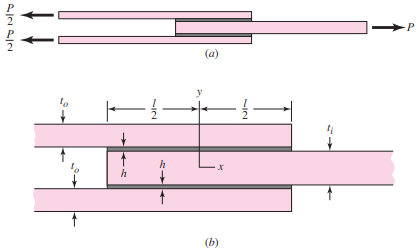
\includegraphics[width=.8\linewidth]{img/adhesion/doubleLap}
	\caption{Analysis of Carbon Fibre Adhesion (From Shigley's Machine Design \cite[484]{shigley})}
	\label{fig:lap}
\end{figure}

The shear-stress distribution of the joint is given by 

\begin{equation} \label{adhesive}
	\tau (x) = \dfrac{P\omega}{4bsinh(\omega l/2)}cosh(\omega x)+\left[\dfrac{P\omega}{4bcosh(\omega l/2)}\left(\dfrac{2E_0t_0-E_it_i}{2E_0t_0+E_it_i}\right)+\dfrac{(\alpha _i-\alpha _0)\Delta T \omega}{(1/E_0t_0+2/E_it_i)cosh(\omega l/2)}\right]sinh(\omega x)
\end{equation}

\begin{equation} \label{omega}
	\omega = \sqrt{\dfrac{G}{h}\left(\dfrac{1}{E_0t_0}+\dfrac{2}{E_it_i}\right)}
\end{equation}

Where $E_o$, $t_0$ $\alpha _0$ and $E_i$, $t_i$ $\alpha _i$ are the modulus, thickness, coefficient of thermal expansion for the outer and inner adherend, respectively. $G, h, b$ and $l$ are the shear modulus, thickness, width and length of the adhesive, respectively. $\Delta T$ is the change in temperature of the joint, from its curing temperature (zero stress temperature). The closer the curing temperature of the adhesive is to the operating temperature, the lower the thermal stresses induced in the joint will be.\\

For this case, an unmodified epoxy will be selected as the adhesive material. From \cite{shigley}, Table 9-7, the lap-shear strength can be anywhere from $10.3-27.6MPa$. $10.3 MPa$ will be selected as a conservative estimate.\\

The outer material is aluminium and the inner material will be carbon fibre. Because of the nature of aluminium, an extremely thin layer of fibreglass should be added between the carbon fibre and aluminium to prevent corrosion due to the curing of the epoxy. Data was found as follows:

\begin{center}
$G=1.3 GPa$ \cite{epoxyShear}\\
$E_i=109GPa$ \cite{carbonFibre}\\
$\alpha _i=23.7*10^{-6}mm/mm^{\circ}C$ \cite{carbonFibre}\\
$E_0=71GPa$ \cite{shigley}\\
$\alpha _0=23.94 mm/mm^{\circ}C$ \cite{shigley}\\
\end{center}

$\Delta T$ can be estimated by assuming the epoxy is cured at room temperature ($20 ^{\circ}C$) and that the lowest temperature the blimp will be used at is  $-40 ^{\circ}C$. This yields $\Delta T = -60^{\circ}C$. The thickness of the adhesive will be estimated as $h=0.5mm$. As preliminary estimates, $t_0= 9.73mm$, $t_i= 9.73mm$, $l=30mm$, and $b=50.80mm$. The force $P$ can be estimated using \textbf{SOME STUFF} $P=100N$.

Substituting these values into Equation \ref{omega} yields
\begin{equation} \label{omegaSolve}
\omega = \sqrt{\dfrac{1300 MPa}{0.5mm}\left(\dfrac{1}{71000MPa*9.73mm}+\dfrac{2}{109000 MPa*9.73mm}\right)} = 0.0930946mm^{-1}
\end{equation}

Followed by substitution into Equation \ref{adhesive}:
\begin{multline} \label{adhesiveSolve}
\tau (x) = \dfrac{100N*0.0930946mm^{-1}}{4*50.80mm*sinh(0.0930946mm^{-1}* 30mm/2)}cosh(0.0930946mm^{-1}* x) + \\ \Bigg[\dfrac{100N*0.0930946mm^{-1}}{4*50.80mm*cosh(0.0930946mm^{-1}* 30mm/2)}\left(\dfrac{2*71000 MPa*9.73mm-1300MPa*9.73mm}{2*71000 MPa*9.73mm+1300MPa*9.73mm}\right)+ \\ \dfrac{(23.7*10^{-6}mm/mm^{\circ}C-23.94*10^{-6} mm/mm^{\circ}C)*(-60^{\circ}C)*0.0930946mm^{-1}}{\left(\dfrac{1}{71000MPa*9.73mm}+\dfrac{2}{109000 MPa*9.73mm}\right)cosh(0.0930946mm^{-1}* 30mm/2)}\Bigg] sinh(0.0930946mm^{-1}* x) \\ = 0.02416MPa*cosh(0.0930946mm^{-1}* x) + [0.02098MPa + 0.1871 MPa]sinh(0.0930946mm^{-1}* x)
\end{multline}

at $x = l/2 = 30mm/2$, the shear is at a maximum value. Therefore, the shear force is $\tau = 0.4464 MPa$, Yielding a safety factor of $\eta = 10.3MPa/0.4464MPa = 23.0734$.

\end{document}